%!TEX root = top.tex
\section{Model}
\label{sec:model}
%In this section, we first review the publicly available model, DeepLab, which we build upon with proposed methods. After that, we introduce the attention model, which weights features at different scales, and then how we further improve the performance by adding extra supervision. 

\subsection{Review of DeepLab}
FCNs have proven successful in semantic image segmentation \cite{dai2015boxsup, liu2015semantic, zheng2015conditional}. In this subsection, we briefly review the DeepLab model \cite{chen2014semantic}, which is a variant of FCNs \cite{long2014fully}. 

DeepLab adopts the 16-layer architecture of state-of-the-art classification network of \cite{simonyan2014very} (\ie, VGG-16 net). The network is modified to be fully convolutional \cite{long2014fully}, producing dense feature maps. In particular, the last fully-connected layers of the original VGG-16 net are turned into convolutional layers (\eg, the last layer has a spatial convolutional kernel with size $\by{1}{1}$). The spatial decimation factor of the original VGG-16 net is 32 because of
the employment of five max-pooling layers each with stride $2$. DeepLab reduces it to 8 by using the {\`a} trous (with holes) algorithm \cite{Mall99}, and employs linear interpolation to upsample by a factor of 8 the score maps of the final layer to original image resolution. There are several variants of DeepLab \cite{chen2014semantic}. In this work, we mainly focus on DeepLab-LargeFOV. The suffix, LargeFOV, comes from the fact that the model adjusts the filter weights at the
convolutional variant of $fc_6$ ($fc_6$ is the original first fully connected layer in VGG-16 net) with {\`a} trous algorithm so that its Field-Of-View is larger. 

%% There are several variants of DeepLab \cite{chen2014semantic}. In this work, we mainly focus on two variants: DeepLab-LargeFOV and DeepLab-MSc-LargeFOV. The suffix, LargeFOV, comes from the fact that the model adjusts the filter weights at the convolutionalized $fc_6$ with {\`a} trous algorithm so that its Field-Of-View is larger. DeepLab-MSc-LargeFOV additionally exploits the features from the intermediate layers for classification (MSc denotes Multi-Scale features) by attaching two-layer MLPs to the image as well as the output of pooling layers to extract multi-scale features. 

\subsection{Attention model for scales}

Herein, we discuss how to merge the multi-scale features for our proposed model. We propose an attention model that learns to weight the multi-scale features. Average pooling \cite{ciresan2012multi, dai2015boxsup} or max pooling \cite{felzenszwalb2010object, papandreou2014untangling} over scales to merge features can be considered as special cases of our method.

\begin{figure}
  \centering   
  \addtolength{\tabcolsep}{-5pt}       
  \begin{tabular}{cc}
   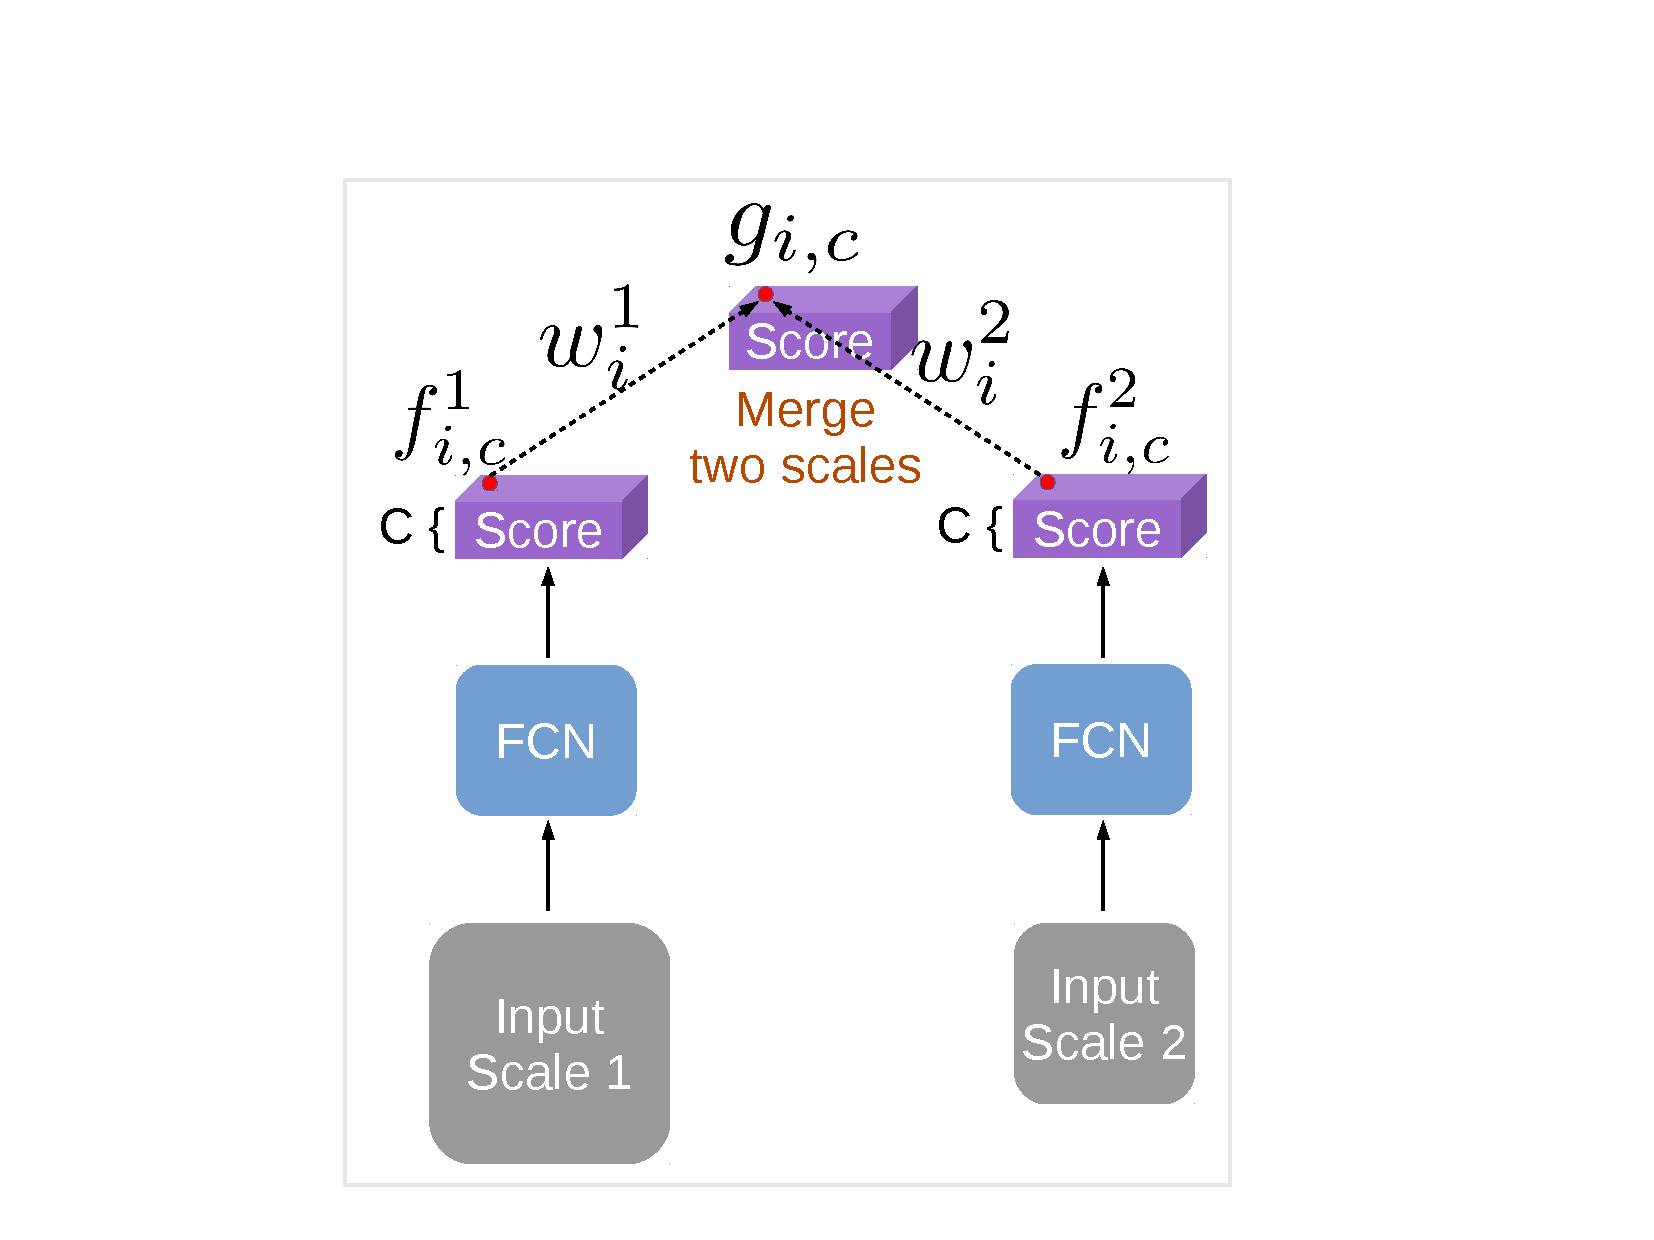
\includegraphics[height=0.53\linewidth]{fig/approach1_2.pdf} &
   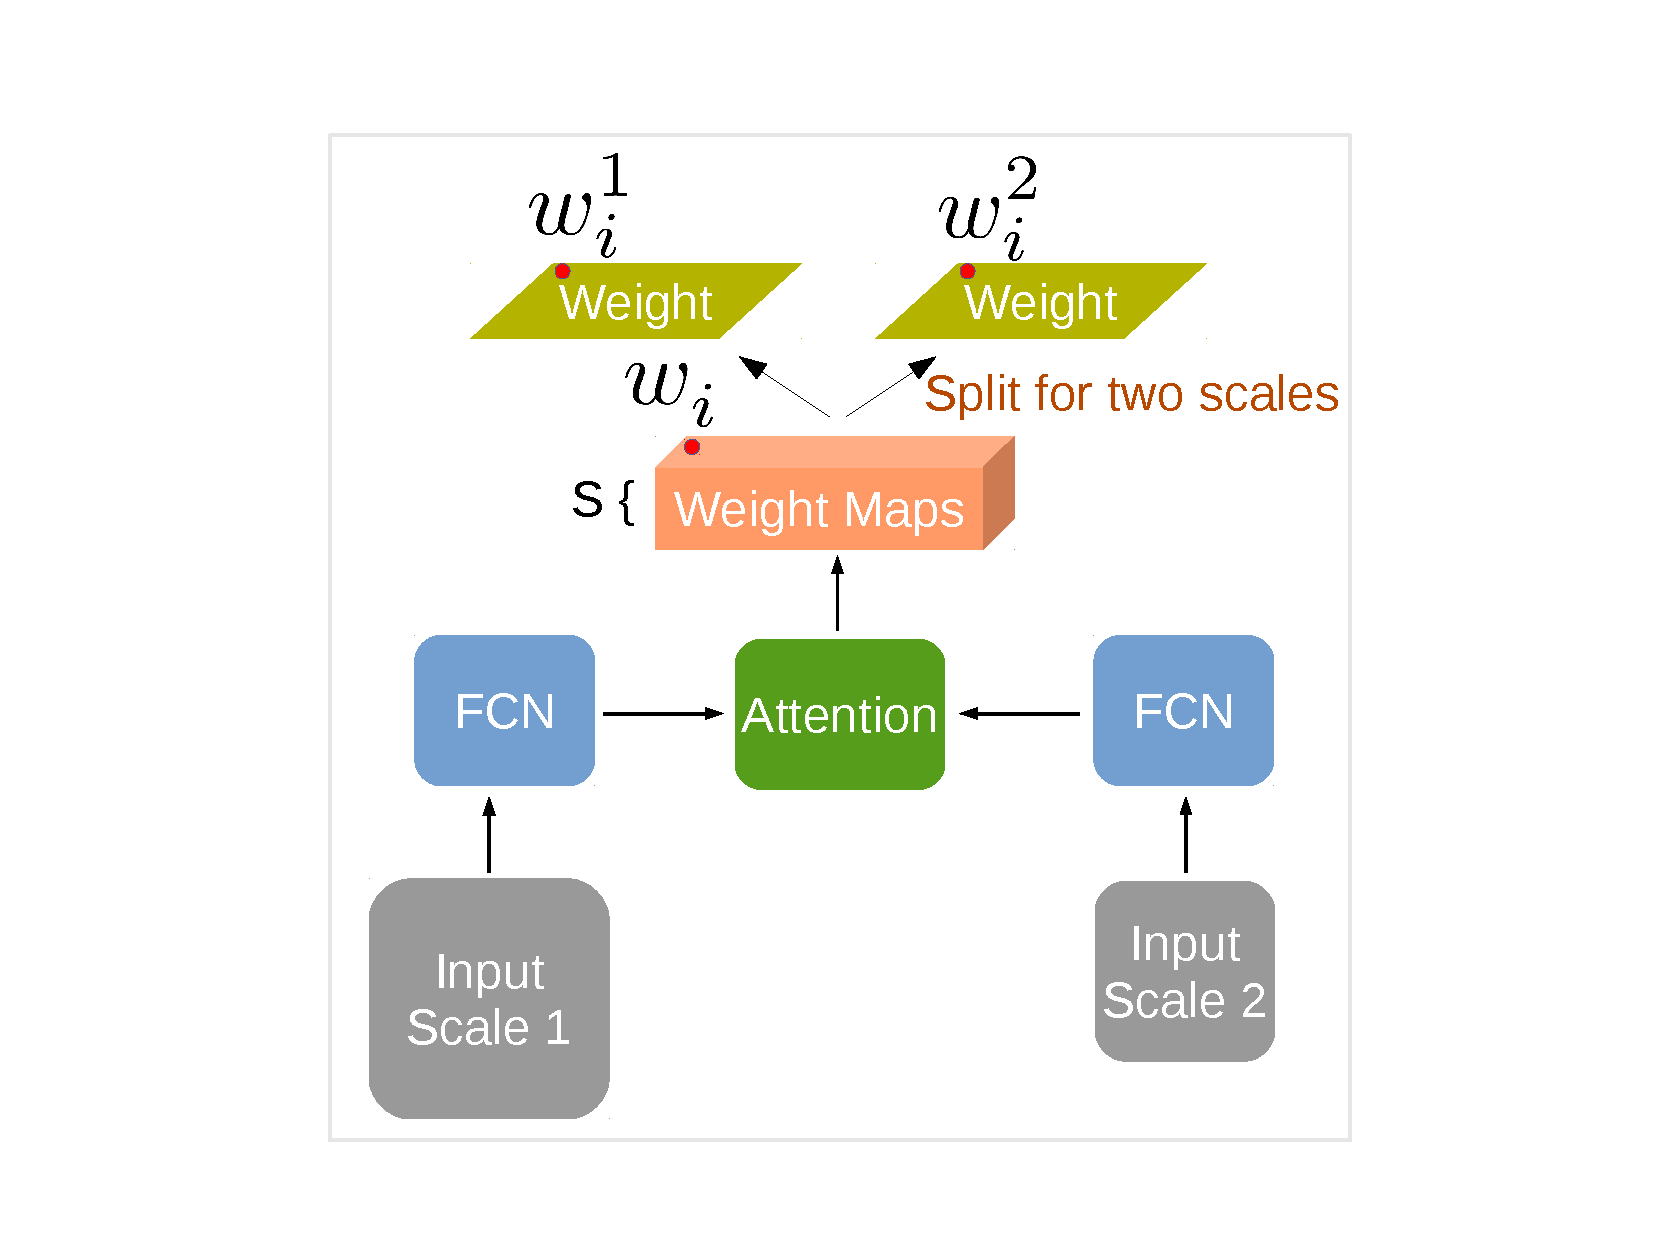
\includegraphics[height=0.53\linewidth]{fig/approach2_2.pdf} \\
   (a)  &
   (b)  \\
  \end{tabular}
  \vspace{1pt}
  \caption{(a) Merging score maps (\ie, last layer output before SoftMax) for two scales. (b) Our proposed attention model makes use of features from FCNs and produces weight maps, reflecting how to do a weighted merge of the FCN-produced score maps at different scales and at different positions.}
  \label{fig:models}
\end{figure}  

Based on share-net, suppose an input image is resized to several scales $s \in \{1, ..., S\}$. Each scale is passed through the DeepLab (the FCN weights are shared across all scales) and produces a score map for scale $s$, denoted as $f^s_{i,c}$ where $i$ ranges over all the spatial positions (since it is fully convolutional) and $c \in \{1, ..., C\}$ where $C$ is the number of classes of interest. The score maps $f^s_{i,c}$ are resized to have the same resolution (with respect to the finest scale) by bilinear interpolation. We denote $g_{i,c}$ to be the weighted sum of score maps at $(i,c)$ for all scales, \ie,

\begin{equation}
\label{eq:weighted_sum}
g_{i,c} = \sum_{s=1}^S w^s_{i} \cdot f^s_{i,c}
\end{equation}

The weight $w^s_{i}$ is computed by
\begin{equation}
w^s_{i} = \frac{\exp(h^s_{i})}{\sum_{t=1}^S \exp(h^t_{i})}
\end{equation}
where $h^s_{i}$ is the score map (\ie, last layer output before SoftMax) produced by the attention model at position $i$ for scale $s$. Note $w^s_{i}$ is shared across all the channels. The attention model is parameterized by another FCN so that dense maps are produced. The proposed attention model takes as input the convolutionalized $fc_7$ features from VGG-16 \cite{simonyan2014very}, and it consists of two layers (the first layer has 512 filters with kernel size $\by{3}{3}$ and second layer has $S$ filters with kernel size $\by{1}{1}$ where $S$ is the number of scales employed). We will discuss this design choice in the experimental results.

The weight $w^s_{i}$ reflects the importance of feature at position $i$ and scale $s$. As a result, the attention model decides how much attention to pay to features at different positions and scales. It further enables us to visualize the attention for each scale by visualizing $w^s_{i}$. Note in our formulation, average-pooling or max-pooling over scales are two special cases. In particular, the weights $w^s_{i}$ in \equref{eq:weighted_sum} will be replaced by $1/S$ for average-pooling, while the summation in \equref{eq:weighted_sum} becomes the $\max$ operation and $w^s_{i}=1 \ \forall s $ and $i$ in the case of max-pooling.

%{\bf Compare with Tu: Generalizing Pooling Functions in Convolutional Neural Networks: Mixed, Gated, and Tree.}

We emphasize that the attention model computes a soft weight for each scale and position, and it allows the gradient of the loss function to be backpropagated through, similar to \cite{bahdanau2014neural}. Therefore, we are able to jointly train the attention model as well as the FCN (\ie, DeepLab) part end-to-end. One advantage of the proposed joint training is that tedious annotations of the ``ground truth scale'' for each pixel is avoided, letting the model adaptively find the best weights on scales.

\subsection{Extra supervision} 
We learn the network parameters using training images annotated at the pixel-level. The final output is produced by performing a softmax operation on the merged score maps across all the scales. We minimize the cross-entropy loss averaged over all image positions with Stochastic Gradient Descent (SGD). The network parameters are initialized from the ImageNet-pretrained VGG-16 model of \cite{simonyan2014very}.

In addition to the supervision introduced to the final output, we add extra supervision to the FCN for each scale \cite{lee2014deeply}. The motivation behind this is that we would like to merge {\it discriminative} features (after pooling or attention model) for the final classifier output. As pointed out by \cite{lee2014deeply}, discriminative classifiers trained with discriminative features demonstrate better performance for classification tasks. Instead of adding extra supervision to the intermediate layers \cite{bengio2007greedy, lee2014deeply, szegedy2014going, xie2015holistically}, we inject extra supervision to the final output of DeepLab for each scale so that the features to be merged are trained to be more discriminative. Specifically, the total loss function contains $1+S$ cross entropy loss functions (one for final output and one for each scale) with weight one for each. The ground truths are downsampled properly \wrt. the output resolutions during training. %In the experimental results, we show that adding extra supervision is essential for merging multi-scale inputs for our proposed methods. 

%% \begin{figure}[!t]    
%%   \centering          
%%   \begin{tabular}{c c c c}
%%    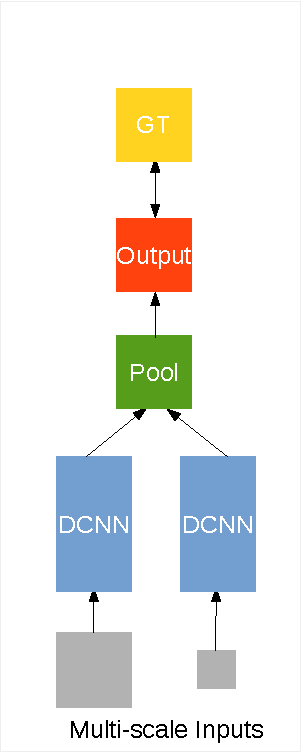
\includegraphics[width=0.2\linewidth]{fig/model1.pdf} &
%%    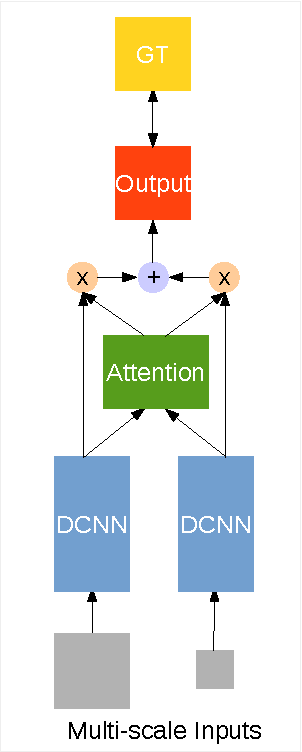
\includegraphics[width=0.2\linewidth]{fig/model2.pdf} &
%%    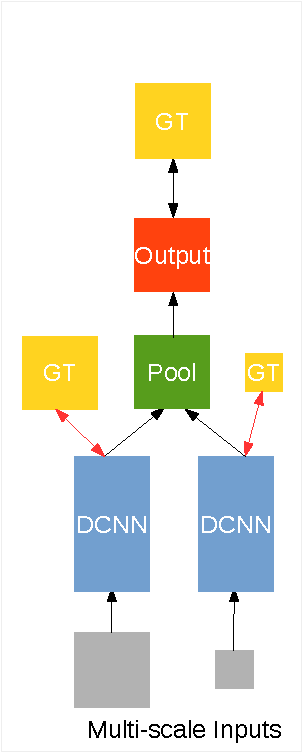
\includegraphics[width=0.2\linewidth]{fig/model3.pdf} &
%%    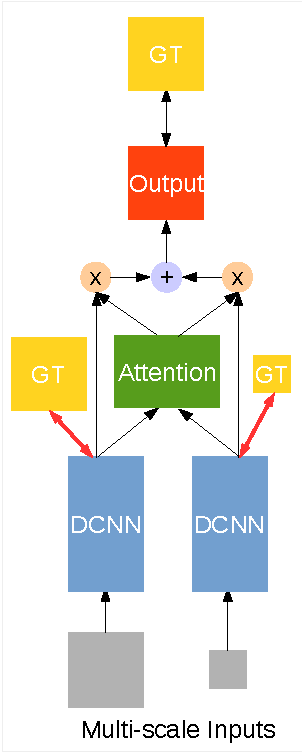
\includegraphics[width=0.2\linewidth]{fig/model4.pdf} \\
%%    (a)  &
%%    (b)  &
%%    (c)  &
%%    (d)  \\
%%   \end{tabular}
%%   \caption{(a): Pooling (either average or max) is employed to merge the multi-scale features. (b): Attention model learns to weight the multi-scale features. (c) and (d): Extra supervision to the DCNN for each scale is added for (a) and (b), respectively. Note that the multi-scale features are resized to the same scale (w.r.t. the finest scale) by bilinear interpolation before merging.}
%%   \label{fig:models}
%% \end{figure}  
